% --------------------------------------------------------------
% This is all preamble stuff that you don't have to worry about.
% Head down to where it says "Start here"
% --------------------------------------------------------------

\documentclass[12pt]{article}

\usepackage[margin=1in]{geometry} 
\usepackage{amsmath,amsthm,amssymb}
\usepackage{graphicx}
\usepackage{caption}
\usepackage{subcaption}

\newcommand{\N}{\mathbb{N}}
\newcommand{\Z}{\mathbb{Z}}

\newenvironment{theorem}[2][Theorem]{\begin{trivlist}
		\item[\hskip \labelsep {\bfseries #1}\hskip \labelsep {\bfseries #2.}]}{\end{trivlist}}
\newenvironment{lemma}[2][Lemma]{\begin{trivlist}
		\item[\hskip \labelsep {\bfseries #1}\hskip \labelsep {\bfseries #2.}]}{\end{trivlist}}
\newenvironment{exercise}[2][Exercise]{\begin{trivlist}
		\item[\hskip \labelsep {\bfseries #1}\hskip \labelsep {\bfseries #2.}]}{\end{trivlist}}
\newenvironment{reflection}[2][Reflection]{\begin{trivlist}
		\item[\hskip \labelsep {\bfseries #1}\hskip \labelsep {\bfseries #2.}]}{\end{trivlist}}
\newenvironment{proposition}[2][Proposition]{\begin{trivlist}
		\item[\hskip \labelsep {\bfseries #1}\hskip \labelsep {\bfseries #2.}]}{\end{trivlist}}
\newenvironment{corollary}[2][Corollary]{\begin{trivlist}
		\item[\hskip \labelsep {\bfseries #1}\hskip \labelsep {\bfseries #2.}]}{\end{trivlist}}

\begin{document}
	
	% --------------------------------------------------------------
	%                         Start here
	% --------------------------------------------------------------
	
	%\renewcommand{\qedsymbol}{\filledbox}
	
	
	\title{Testing Different Vectorization Techniques on Persistence Diagrams and Their Effect on the Clustering of the Data \\   \large  Topological Data Analysis - group project}
	\author{%replace with your name
		Bernarda Petek, Jon Selič} %if necessary, replace with your course title
	
	\date{16.1.2023}
	\maketitle
	
	
	
\section{Introduction}
Topological data analysis (TDA) is a modern tool for data analysis which can be used in many different ways. Even though the community is generally agreed on a standard TDA pipeline, many decisions still have to be made by the analyst which can greatly affect the results and their interpretation. In this project we applied five different variations of the TDA pipeline and compare their results.

\section{Data and Methods}
\subsection{Obtaining Pointclouds}
Data was obtained from two different sources, Our World in Data\footnote{https://ourworldindata.org/} and Data World Bank\footnote{https://data.worldbank.org/}. For each country with at least one year of data, we obtained the GDP per person employed, total population, refugee population, percentage of people enrolled in primary school, and total number of working people throughout the years 1960-2021. We filter the data by removing the rows with missing parts of data. We also filter the data by removing the countries which had less than 26 years worth of data. For every country we used the data from 1995 to 2020.

So for each country we got 26 years worth of data which consisted of GDP per person employed, population, refugee population, percentage of people enrolled in primary school, and total number of working people. We then standarize the data. Finally, to get pointclouds, we partition the data by countries. 

\subsection{Filtration and Computing Persistent Homology}
Next, we compute the persistent homology for each point-cloud and represent it with a persistence diagram. To do this, we first have to build a filtration on a simplicial complex constructed on the points in the pointcloud. For building Vietoris-Rips filtration and computing persistent homology we use the Ripser.py library. For each pointcloud we compute $0$ and $1$ dimensional persistent homology groups. We limit ourselves to these dimensionas as higher dimensions are usually harder to compute. Before computing the persistent homologies on our point-clouds we validated our approach on dummy data. We made a few pointclouds where every point had four random coordinates ranging from $1$ to $100$. We computed the persistent homology up to dimension $3$. Computing persistent homology for dimensions $2$ and $3$ indeed took a long time. However, we observed that random dummy data had some one- and even two- dimensional holes. Then when we computed persistent homology on some of our data we realized our data is usually shaped in a way that there are no holes. Subsequently we realized that in our case we only needed to compute $0$ dimensional persistent homology and its persistence diagram. That made sense because our data was linearly changing through the time. So we computed 0 dimensional persistent homology and  represented it with persistence diagram for each pointcloud. 

\subsection{Space of Persistence Diagrams and Clustering}
After computing the $0$-dimensional persistent homology for every point-cloud, we obtain a space of persistence diagrams. We compute two different distance matrices for two different distance metrics on the space of persistence diagrams. For the first distance matrix, we used bottleneck distance between persistence diagrams and for the second distance matrix we used the Wasserstein distance between the persistence diagrams. After computing the distance matrices we use agglomerative clustering on the space of the persistence diagrams to find similarities between our point-clouds. We link persistence diagrams which were put together by the clustering algorithm to the original point-clouds. By using helper function plot\_dendrogram from the scikit-learn library we obtain two different dendrograms, each showing the similarities and differences between the shape of the countries data with the help of their persistence diagrams.

\subsection{Vectorization and Clustering}
In the next step, we extended our pipeline by vectorizing the data from the persistence diagrams before using it in a clustering algorithm. We did this in two ways: Firstly, by computing the component weights for the Gaussian mixture model (GMM) that has been trained on all of our diagrams and computing the distance between them - and secondly, transforming the persistence diagram into a pixelated persistence image and computing the distance between each pixel in the transformed image. The distance between two images was computed in two different ways: A simple euclidean distance metric, taking the flattened images as input vectors, and the average mean squared error (MSE) between the pixels of the two images. The resulting two distance matrices were then used in the clustering algorithm, similarly as in the previous step. The result was three additional dendrograms.

\section{Results}
The dendrogram of the clustering made on persistence diagrams with bottleneck distance can be seen on Figure 1. Countries were put into 24 different clusters, for example ['Costa Rica', 'Kyrgyzstan', 'Nicaragua', 'Paraguay', 'Peru', 'Philippines', 'Slovenia', 'South Africa', 'Togo', 'United Kingdom', 'Uzbekistan']. The dendrogram of the clustering made on persistence diagrams with Wasserstein distance can be seen on Figure 2. Countries were put into 29 different clusters, for example ['Albania', 'Algeria', 'Argentina', 'Belarus', 'Czechia', 'Italy', 'Malaysia', 'Paraguay', 'Slovenia', 'South Korea', 'Thailand', 'United Kingdom']. The intersection of those two clusters consists of  Paraguay, Slovenia and United Kingdom, which is not a lot. However, even though those countries weren't in the same clusters, they were quite close in both dendrograms. What is more interesting
is that some of the countries that we did not expect were clustered together, for example ['Burkina Faso', "Cote d'Ivoire", 'Luxembourg', 'Niger']. Burkina Faso, Cote d'Ivoire and Niger are all countries in West Africa and they all used to be French colonies. It is interesting that the shape of their data from the past 26 years is the same as the shape of Luxembourg's data from the past 26 years. While this may be a simple case of correlation, it may nonetheless be an interesting coincidence.

\begin{figure}[t]
	\centering
	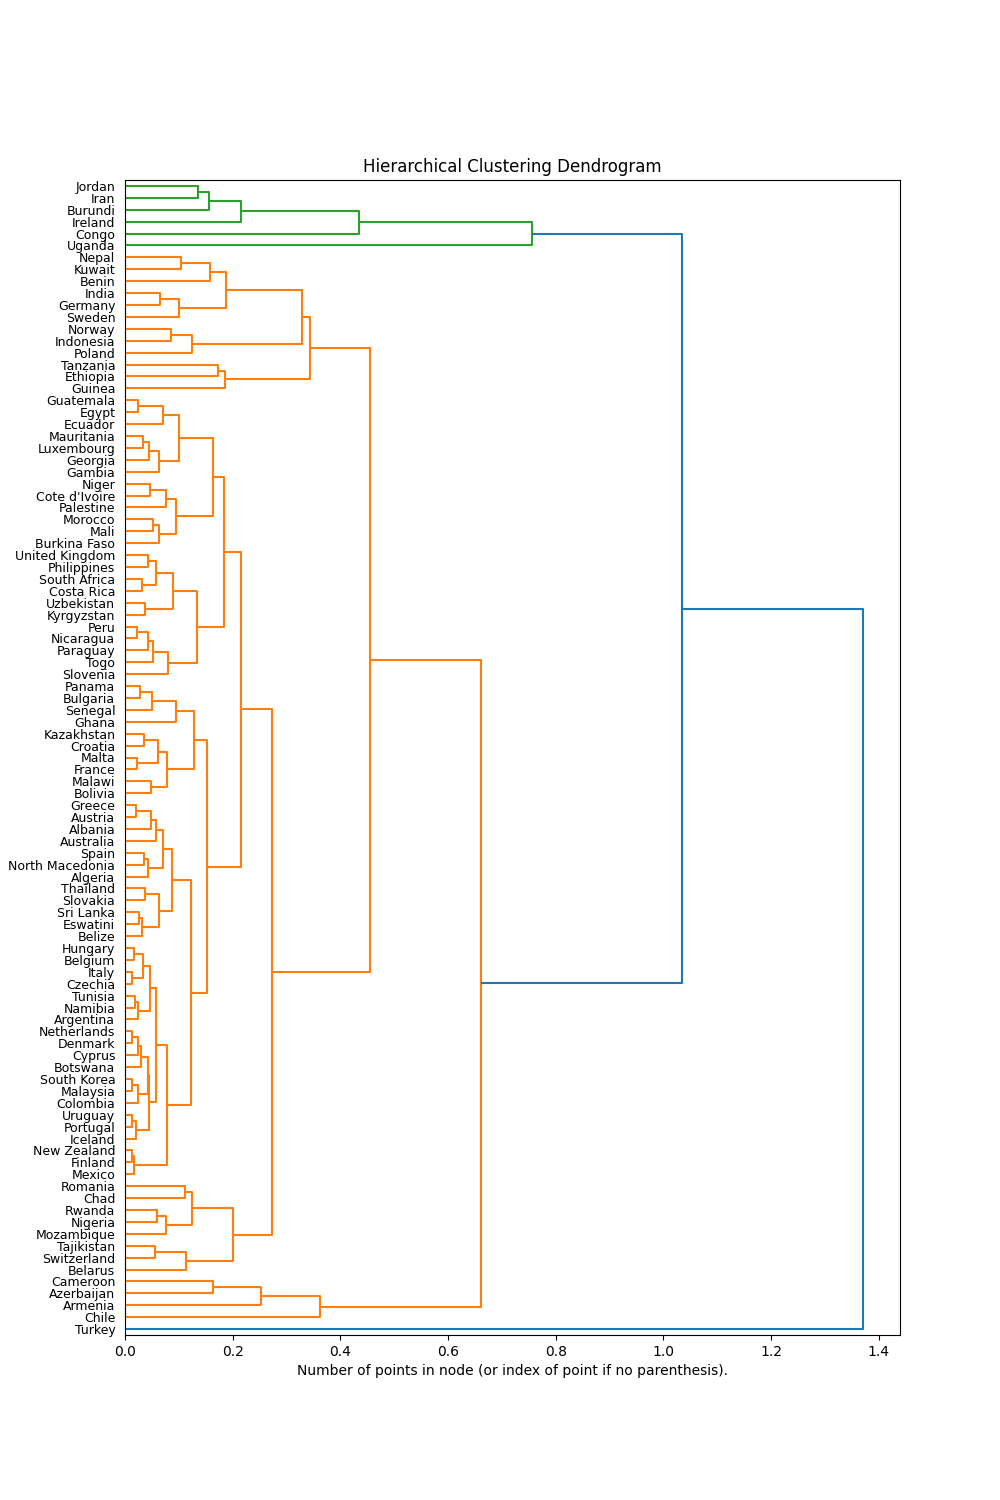
\includegraphics[width=15cm]{bottleneck.png}
	\caption{Dendrogram based on bottleneck distance between persistence diagrams.}
\end{figure}

\begin{figure}[t]
	\centering
	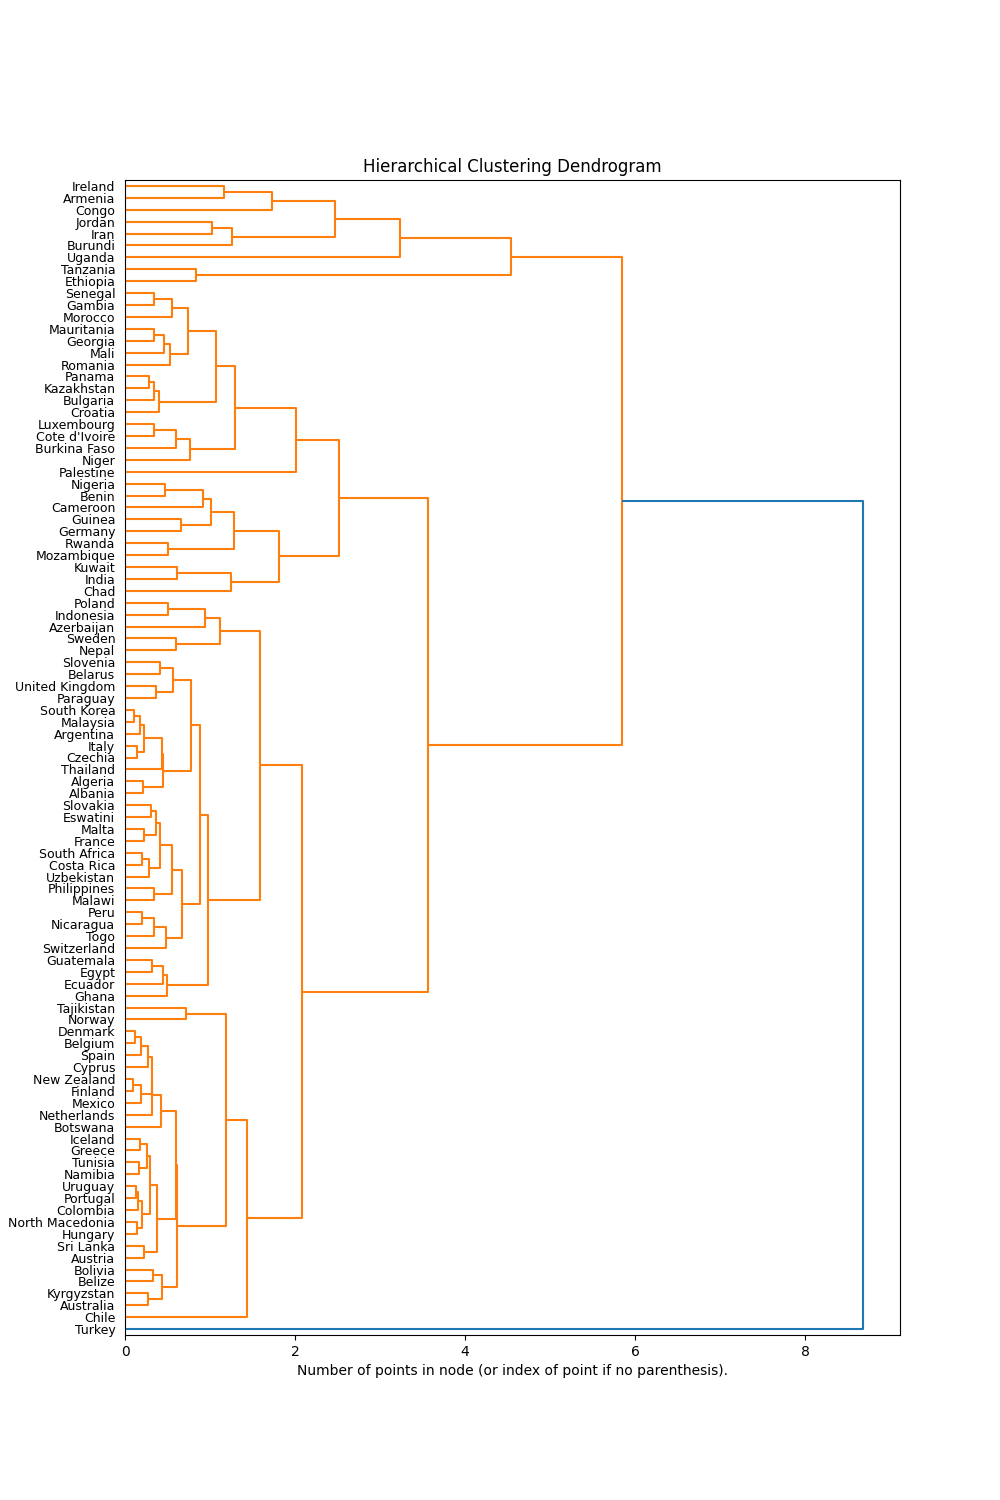
\includegraphics[width=15cm]{wasserstein.png}
	\caption{Dendrogram based on Wasserstein distance between persistence diagrams.}
\end{figure}

\section{Conclusion}


\section{Division of Work}
Bernarda obtained, filtered, and preprocessed the data. She performed filtration, computing the persistent homology, and tested two different clustering approaches on the space of persistence diagrams.

Jon tested three different vectorizations of the persistent diagrams, and applied clustering in the Euclidean space on the obtained vectorizations. 
	% --------------------------------------------------------------
	%     You don't have to mess with anything below this line.
	% --------------------------------------------------------------
	
	
\end{document}    
